\documentclass{beamer}
\usepackage{fancybox}
\usepackage{beamerthemesplit}
\usepackage{hyperref}

\mode<presentation> {

\usetheme{Warsaw}
\setbeamertemplate{footline}[frame number]

  }
\title[Updated stock-recruitment DB]{The RAM II stock-recruitment database}
\subtitle{An historical and technological overview}
\author[Baum, Jensen, Minto and Ricard]{Julia Baum \thanks{Scripps Institution of Oceanography, UCSD} \and Olaf Jensen \thanks{University of Washington} \and Coil\'{i}n Minto \thanks{Dalhousie University, Halifax NS, Canada} \and Daniel Ricard$^{3}$}

\date{Nov. 2nd 2009 - UW SAFS - Hilborn/Punt/Essington labs}

\begin{document}


\frame{\titlepage}
% [plain]


%\frame{\tableofcontents}

\section{Past}

\begin{frame}
\frametitle{RAM's original database}

\begin{itemize}
 \item A lifelong endeavour that started when RAM worked at DFO
 \item First summarised in a technical report and resulted in numerous publications
 \item Focused on:
\begin{itemize}
 \item Meta-analytical methods to draw strength from many stocks
 \item The relationship between spawning stock and recruitment 
 \item Maximum reproductive rate at low spawning stocks
\end{itemize}
 \item Housed in flat text files and handled by a variety of scripts (mostly Perl, SPlus and SAS)
\end{itemize}

Archived on server (i.e not updated anymore) and available from the following URL:\\
\url{http://chase.mathstat.dal.ca/~myers/welcome.html}

\end{frame}


\section{Present}
\begin{frame}
\frametitle{RAM II database - srdb}
\begin{itemize}
 \item A user-built database
 \item A relational database using the Open Source postgreSQL RDBMS with postGIS
 \item Internet accessible (TCP/IP), concurrent users, privileges and credentials
 \item Data from individual assessments are captured in a standardised spreadsheet file
 \item Suite of Open Source tools used for development (BASH, Perl, LaTeX, R, Python)
 \item Under version control using the Open Source Subversion system

% \item Still under active development with more assessments being added and probably some design changes
\end{itemize}

\end{frame}


\begin{frame}[plain]
\frametitle{Database structure - Entity relationship diagram}
\hspace*{-.6cm} 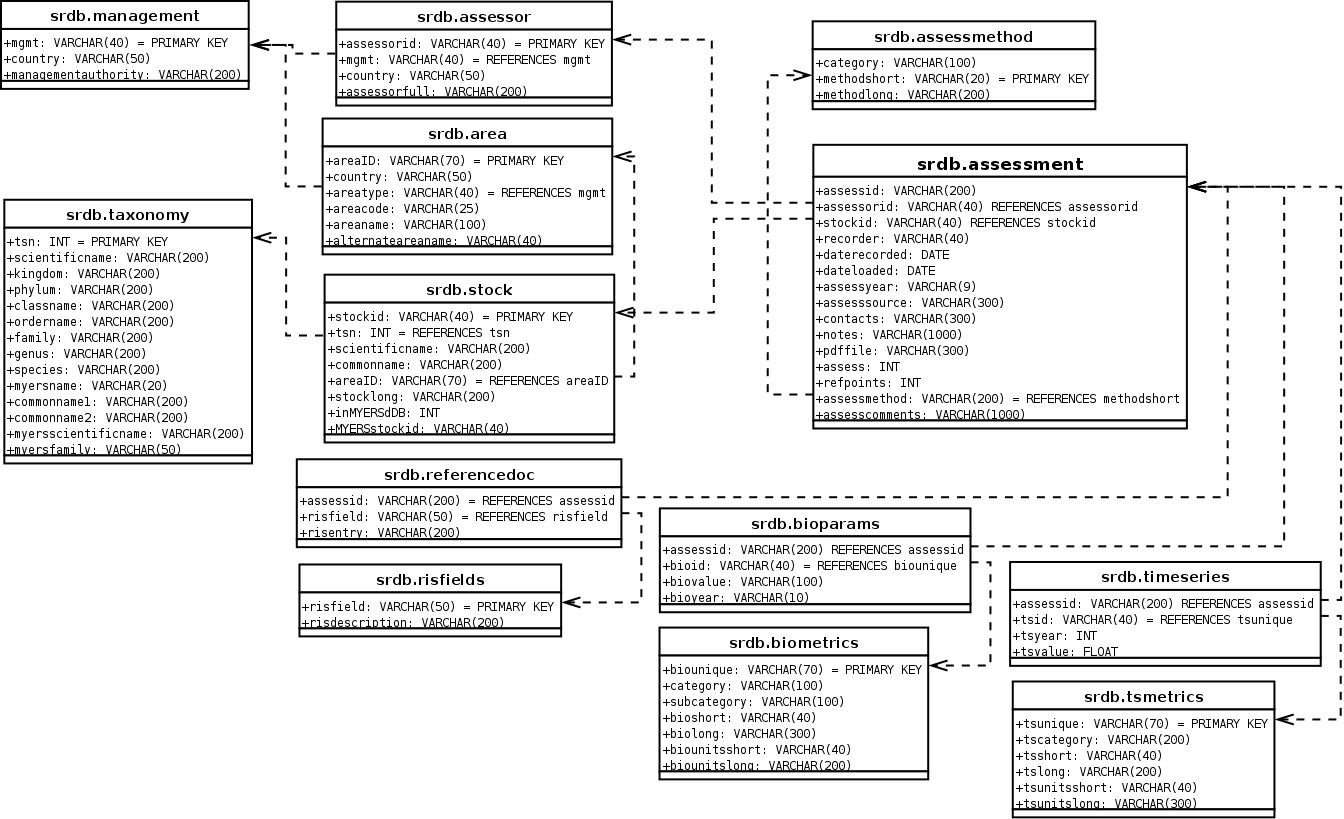
\includegraphics[scale=0.18]{/home/srdbadmin/SQLpg/srdb/trunk/doc/srdb-ERD.png}
\end{frame}

%\begin{frame}
%\frametitle{Summary of database content, as of Dec. 10$^{\textnormal{th}}$ 2008}
% tot. num assessments by recorder, taxonomic order
% Geographic coverage (map)
% keep simple
%Changes daily whilst under active development
%\end{frame}

\begin{frame}[plain]
\frametitle{Geographic coverage}
\begin{center}
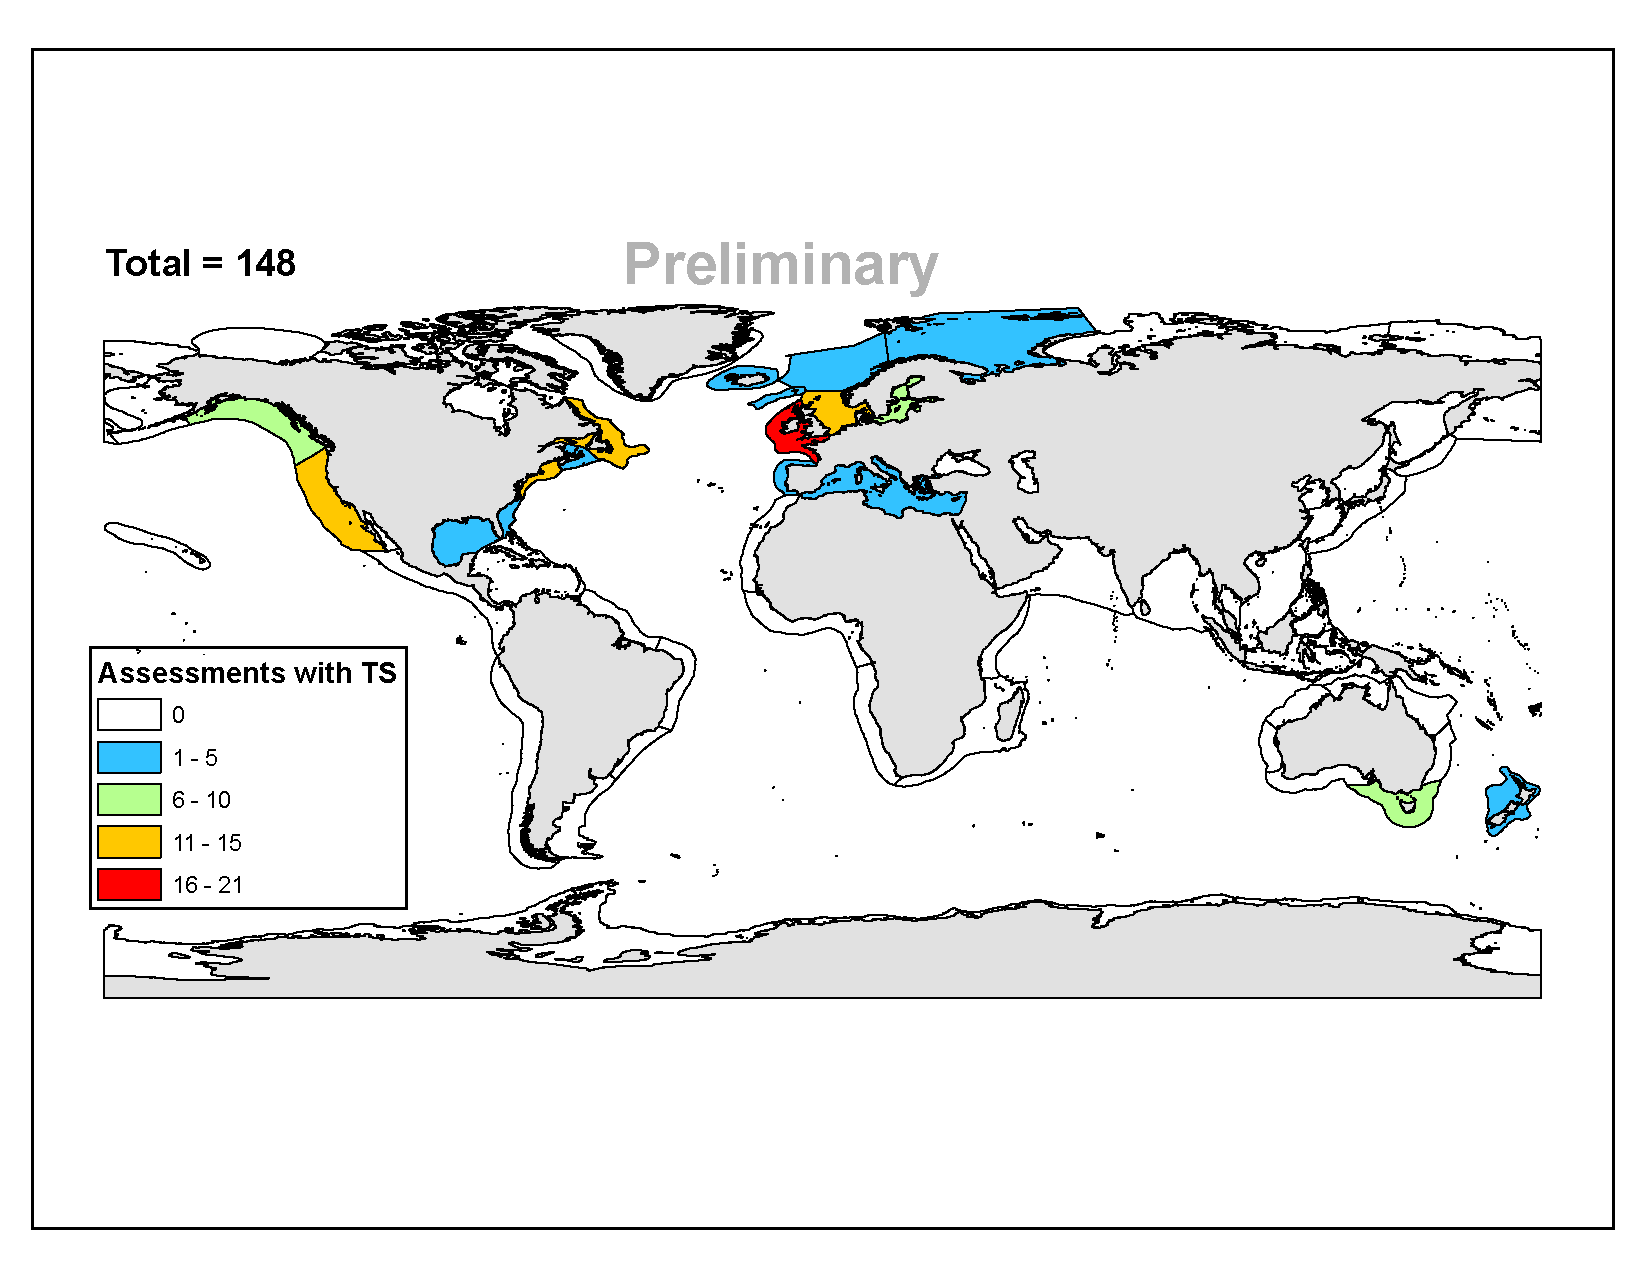
\includegraphics[width=10cm]{/home/srdbadmin/SQLpg/srdb/trunk/doc/Data_summary_by_LME.pdf}
\end{center}
\end{frame}

\begin{frame}[plain]
\frametitle{Number of entered assessments}
\begin{center}
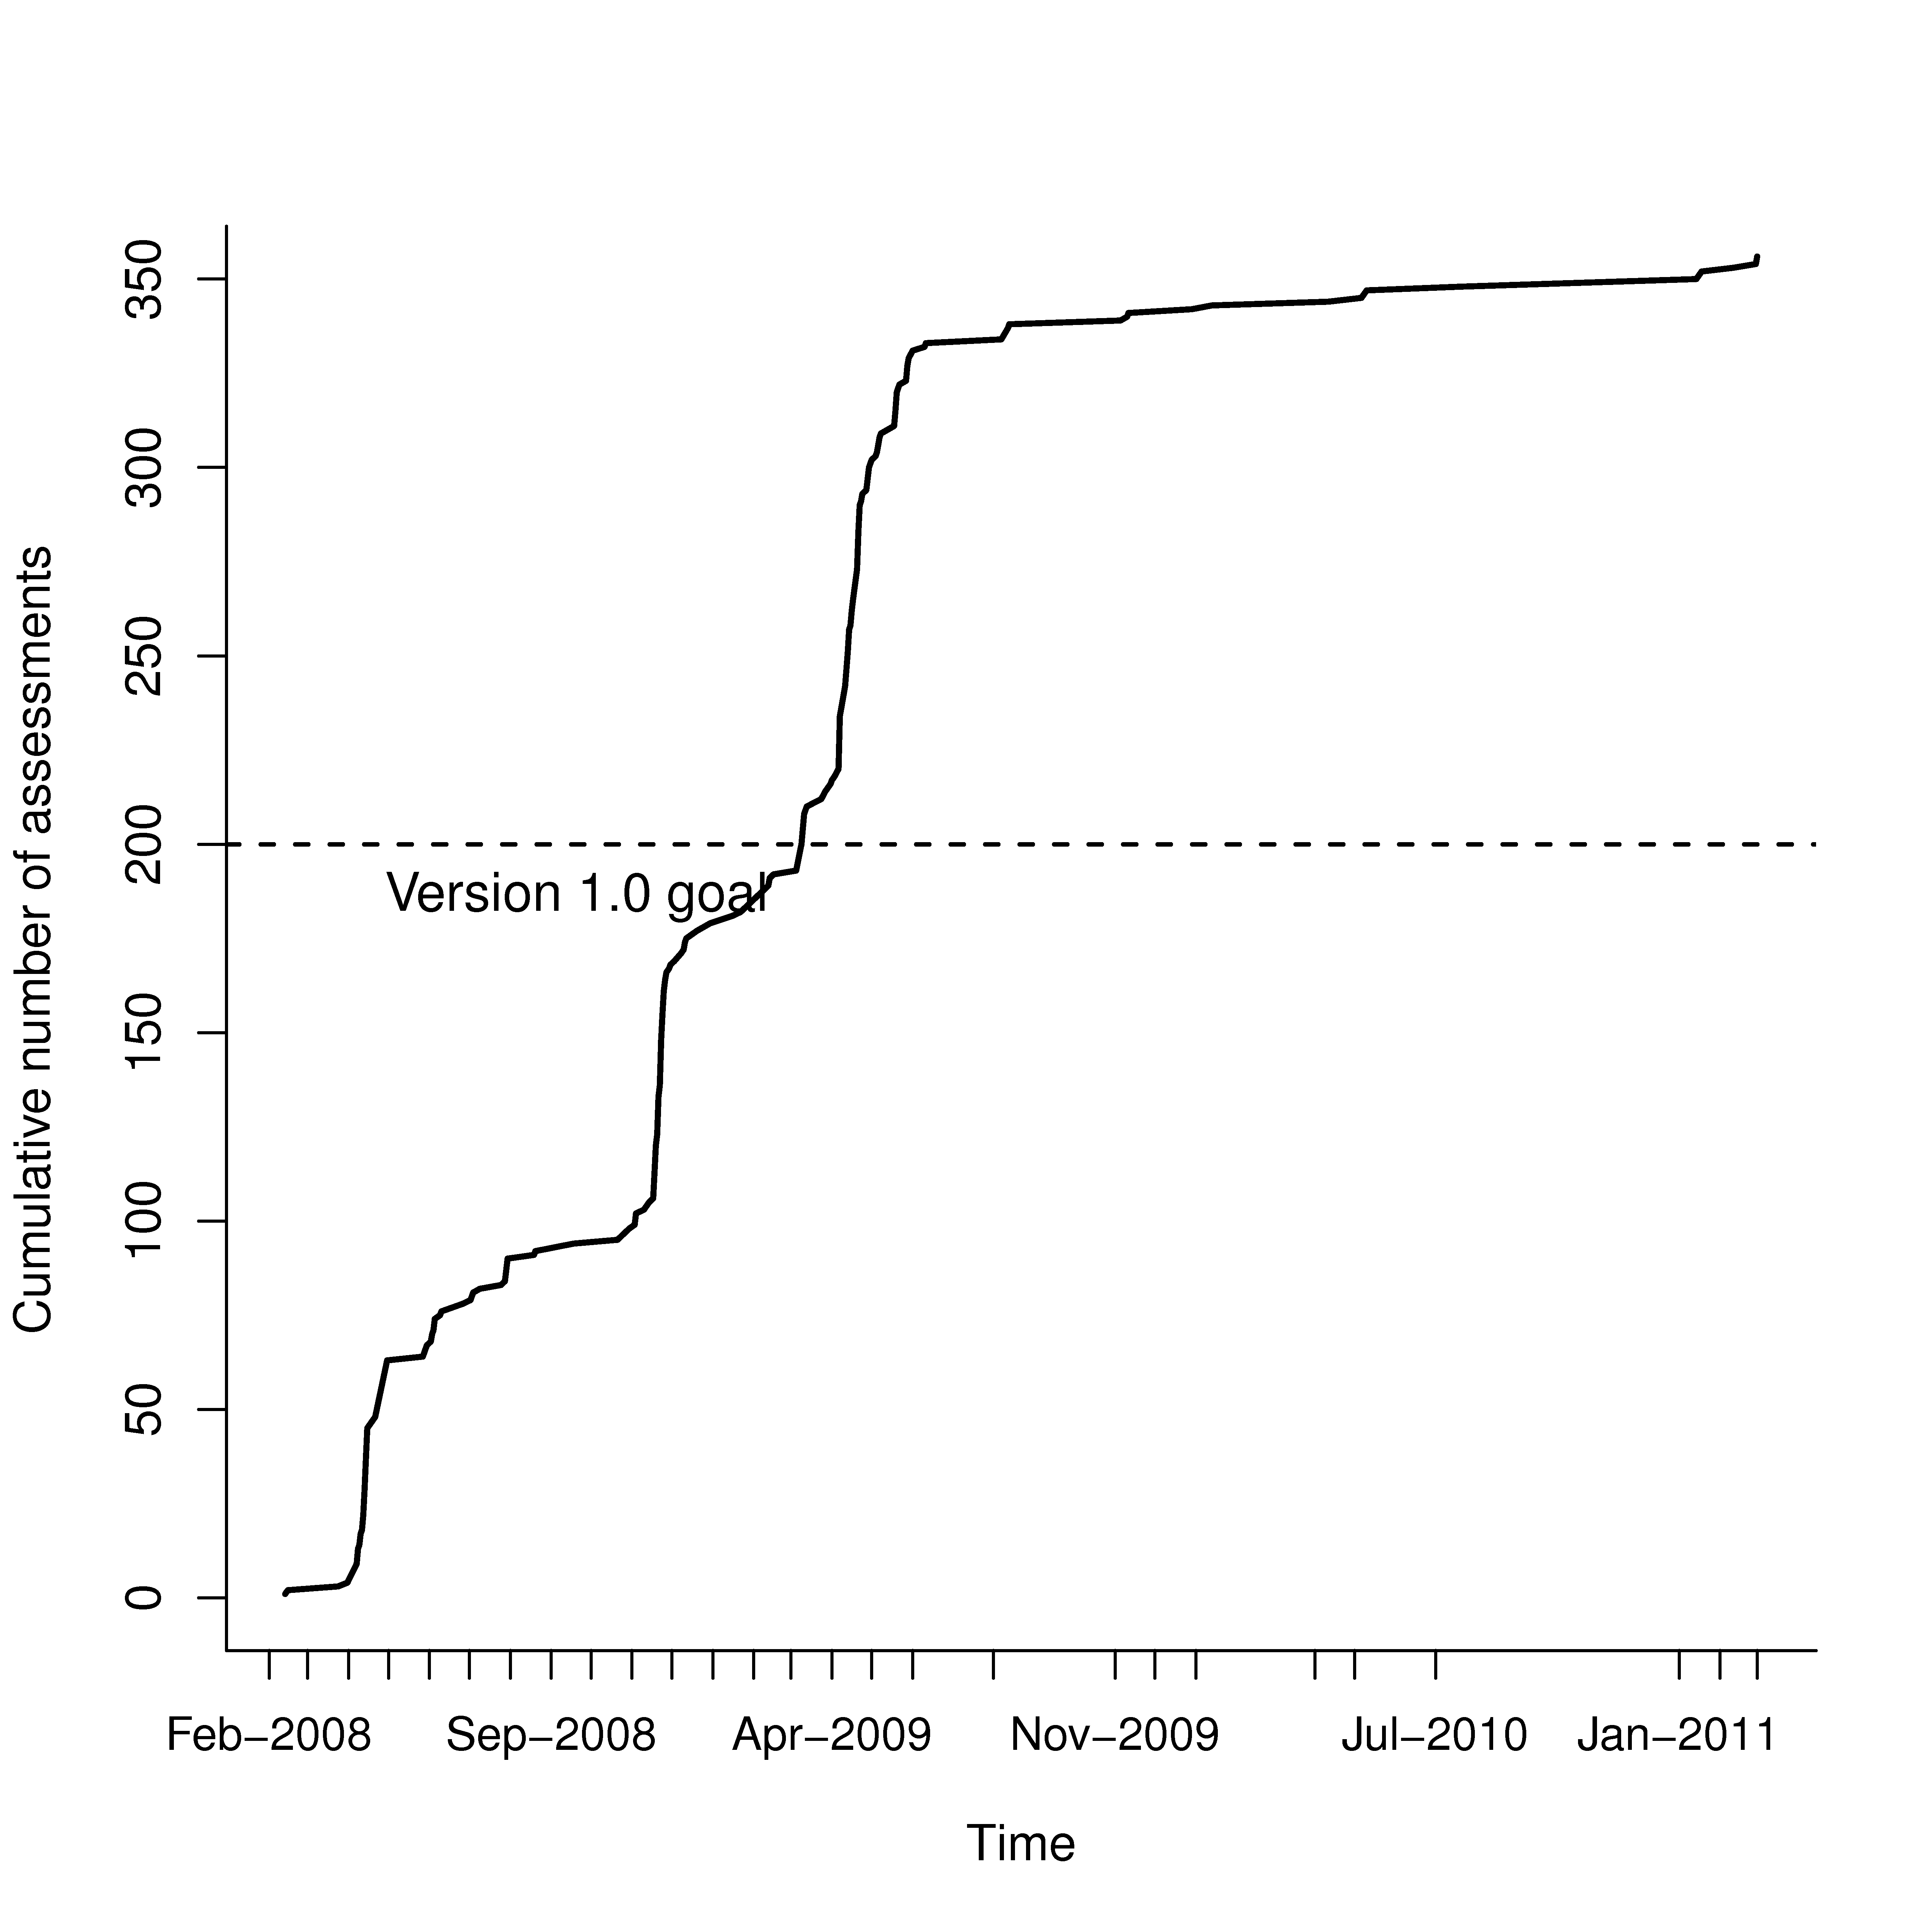
\includegraphics[width=8cm]{/home/srdbadmin/SQLpg/srdb/trunk/doc/timeseries_assess.png}
\end{center}
\end{frame}

\begin{frame}
\frametitle{Demo session}
RAMlegacy portal: \url{http://www.marinebiodiversity.ca/RAMlegacy}\\
\vspace{.5cm}
How to:
\begin{enumerate}
\item Submit an assessment
\item Track assessment progress
\item Connect to the database on
\begin{itemize}
\item[-] development server
\item[-] local machine from UW
\end{itemize}
\item Get timeseries data in R and plot SSB and F
\item SSB temporal trends pre- and post-1992
\item Generate a QAQC document using Perl script
%\item Plot the timeseries data %QC/QA script (run perl script)
\end{enumerate}
\end{frame}

\section{Future}

\begin{frame}
\frametitle{Release of srdb version 1.0}
Points to consider before wider distribution and usage:
\begin{itemize}
 \item How to make this data authoritative? {\bf QC/QA}
 \item How to make this data citable? {\bf Metadata and summary publication}
 \item How to make analyses reproducible? {\bf Versioning of database content}
 \item How to ensure usability? {\bf Documentation, tailored database views as data products for users}
 %\item Data access decisions? 
\end{itemize}
\vspace{.25cm}
Complete entry of top-twenty tonnage fisheries\\
\vspace{.25cm}
Anticipated formal release: {\bf early 2010}\\
Submit manuscript and copy database to production server at Dalhousie
\end{frame}

\begin{frame}
\frametitle{Longterm plans}
\begin{itemize}
\item Addition of stocks from other areas (Africa, South America, Asia), 
\item Addition of new species (salmonids, freshwater fishes, invertebrates)
\item Addition of ancillary data (management, economic, life history data.....)
\item Engage with regional fisheries agencies for timely inclusion of new assessments 
\item Ensure appropriate linkages with other global fisheries-related databases (Fishbase, SAUP, FAO catch statistics) 
% \item Develop a web-based interface for querying the database
\end{itemize}
\end{frame}

\begin{frame}
\frametitle{Acknowledgments}
Sincere thanks to:\\
\vspace{.5cm}
RAM \\
All assessment scientists\\ 
All recorders\\
NCEAS working group and DGS
\end{frame}
\end{document}
